\myChapter{Généralités sur le Business Process Model and Notation et applications web métier}{}
\label{chap:services_composition_generalities}
\myMiniToc{mysection}{Sommaire}

\mySection{Introduction}{}

Dans ce chapitre, nous présentons les notions de base nécessaires à la
compréhension de notre travail. Nous abordons dans un premier temps les processus
métier, le BPM et BPMN. Dans un second temps, nous rappelons les concepts du
développement web utiles à l'étude des applications métier. Cette
présentation permet de préciser le lien entre modèle métier, moteur de processus
et application web.

\mySection{Processus métiers et gestion des processus métiers (BPM)}{}
\label{sec:calcul_orientee_service}

\subsection{Processus métier}{}
\label{subsec:evolution_high_performance}

Un processus peut être compris comme un ensemble d'activités corrélées qui transforment des éléments d'entrée en éléments de sortie. Cette définition, proche de celle de l'ISO 9000, met l'accent sur l'enchaînement, la transformation et le résultat attendu. Hammer et Champy définissent également le processus comme un ensemble finalisé d'activités produisant une valeur pour un client \cite{hammer1993}.
%Pour bien définir le processus métier, voici quelques définitions de processus.
%\begin{itemize}
    %\item Un processus est défini par l'ISO 9000 (2000) comme un 
    %\og ensemble d'activités corrélées ou interactives qui transforme des éléments d'entrée en éléments de sortie \fg.

   % \item La définition générale proposée par le \textit{Petit Robert} est :
    %\og un processus est un ensemble de phénomènes conçus comme actifs et organisés dans le temps \fg.

   % \item Pour l'Association française de normalisation (AFNOR) :
    %\og un processus est une succession d'activités réalisées à l'aide de moyens 
    %(personnel, équipement, matériels, informations) et dont le résultat final attendu est un produit \fg.

    %\item M. Hammer et J. Champy, en 1993, décrivent un processus comme un 
    %\og ensemble finalisé d'activités, orientées vers la production d'un résultat représentant une valeur pour un client \fg.
%\end{itemize}

Un processus métier est un processus lié à un objectif concret de l'organisation. Il décrit comment une structure produit un service, traite une demande, prend une décision ou coordonne plusieurs intervenants.

Le caractère métier du processus est important. Le processus exprime d'abord une réalité organisationnelle avant de devenir une réalité informatique. Il précise ce qui doit être fait, par qui, avec quelles informations, selon quelles règles et avec quel résultat.

Un processus métier comporte généralement trois dimensions. La dimension fonctionnelle répond à la question : que faut-il faire ? La dimension organisationnelle répond à la question : qui le fait ? La dimension informationnelle répond à la question : quelles données sont nécessaires ou produites ? Ces trois dimensions forment une base utile pour passer ensuite vers la conception d'un système d'information.
\begin{table}[H]
\centering
\caption{Composantes essentielles d'un processus métier}
\begin{tabularx}{\textwidth}{p{3cm}X}
\toprule
\textbf{Composante} & \textbf{Rôle dans le processus}\\
\midrule
Entrées & Éléments nécessaires au démarrage ou à l'exécution : demande, formulaire, document, événement ou information reçue.\\
Activités & Opérations réalisées par des acteurs humains ou des systèmes.\\
Acteurs & Personnes, services, rôles ou applications responsables des activités.\\
Règles & Conditions qui orientent l'exécution, les décisions, les validations et les autorisations.\\
Sorties & Résultats produits : dossier validé, demande rejetée, document généré, notification envoyée.\\
\bottomrule
\end{tabularx}
\end{table}
\begin{figure}[H]
\centering
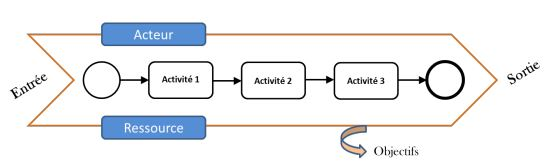
\includegraphics[width=0.75\textwidth]{Chap1/images/image1.JPG}
\caption{Exemple de processus métier }
\label{fig:chap2-ifml-symfony}
\end{figure}

\subsection{Gestion des processus métier (BPM)}

\subsubsection{Définitions de la gestion des processus métier}

Plusieurs définitions ont été données pour le terme de gestion des processus métier.

D'après  Van Der Aalst et al. , le \textit{Business Process Management} (BPM) comprend
\og les méthodes, les techniques et les outils permettant de concevoir, d'exécuter, de gérer et d'analyser les processus opérationnels, en s'appuyant sur des acteurs pouvant être des êtres humains, des organisations, des applications et d'autres sources d'information \fg \cite{vanderAalst2003bpm}.

Le \textit{Business Process Management} (BPM) peut également être défini comme l'art de modéliser, de gérer et d'optimiser les processus métiers afin d'améliorer la performance des entreprises. Il nécessite l'utilisation d'outils permettant de modéliser, d'intégrer, de superviser et d'analyser le fonctionnement des processus tout au long de leur cycle de vie, dans une logique d'amélioration continue \citep{dumas2018fundamentals,weske2012bpm}.
\subsection{Cycle de vie du BPM}

Selon Marlon Dumas \citep{dumas2013fundamentals}, le BPM peut être considéré comme un cycle continu comprenant les phases suivantes
\begin{figure}[H]
\centering
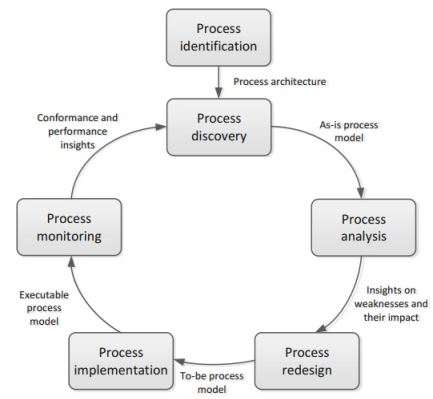
\includegraphics[width=0.75\textwidth]{Chap1/images/image2.JPG}
\caption{Cycle de vie du BPM \citep{dumas2013fundamentals} }
\label{fig:chap2-ifml-symfony}
\end{figure}

\subsubsection{Identification du processus \textit{(Process Identification)}}

Cette étape part d’un problème concret rencontré dans l’entreprise. Il s’agit alors de repérer les processus concernés, d’en préciser les limites et de comprendre les liens qu’ils entretiennent avec les autres processus. Ce travail conduit à une architecture de processus, nouvelle ou actualisée, qui donne une vue d’ensemble du fonctionnement de l’organisation. Cette architecture sert ensuite de base pour choisir le ou les processus qui seront traités dans les autres phases du cycle de vie. L’identification des processus s’accompagne souvent de la définition des indicateurs de performance.

\subsubsection{Découverte des processus \textit{(Process Discovery)}}

Cette phase correspond à la description de la situation existante. Elle consiste à représenter le fonctionnement réel des processus retenus, le plus souvent à travers un ou plusieurs modèles de processus. Elle permet ainsi de disposer d’une vision claire de la manière dont le travail est effectivement réalisé.

\subsubsection{Analyse du processus \textit{(Process Analysis)}}

À ce niveau, les difficultés liées au processus sont relevées, décrites et, lorsque cela est possible, mesurées à l’aide d’indicateurs de performance. Le résultat obtenu est une liste organisée des problèmes constatés. Ces problèmes sont ensuite hiérarchisés selon leur importance, leur impact sur le processus et l’effort nécessaire pour les corriger.

\subsubsection{Refonte du processus \textit{(Process Redesign)}}

Cette phase, aussi appelée amélioration du processus, vise à proposer les modifications capables de résoudre les problèmes identifiés précédemment et d’aider l’organisation à atteindre ses objectifs de performance. Plusieurs possibilités de changement sont étudiées, puis comparées à partir des indicateurs retenus. Ainsi, la refonte reste étroitement liée à l’analyse : chaque solution envisagée doit être évaluée avant d’être retenue. Les options les plus pertinentes sont finalement regroupées pour produire un processus amélioré, généralement présenté sous forme de modèle.

\subsubsection{Mise en œuvre du processus \textit{(Process Implementation)}}

Cette étape consiste à préparer et à appliquer les changements permettant de passer du processus actuel au processus cible. Elle comporte deux dimensions principales : le changement organisationnel et l’automatisation. Le changement organisationnel concerne l’adaptation des pratiques de travail des acteurs impliqués dans le processus. L’automatisation, quant à elle, renvoie à la mise en place ou à l’amélioration des systèmes informatiques destinés à soutenir le nouveau processus.

\subsubsection{Suivi du processus \textit{(Process Monitoring)}}

Lorsque le processus amélioré est exécuté, des données sont collectées puis analysées afin d’évaluer sa performance par rapport aux objectifs fixés. Cette observation permet de détecter les lenteurs, les erreurs fréquentes ou les écarts par rapport au fonctionnement prévu. Des actions correctives peuvent alors être engagées. De nouveaux problèmes pouvant apparaître dans le même processus ou dans d’autres, le cycle BPM doit être repris de manière continue.

\subsection{Systèmes de gestion des processus métiers}

Les systèmes de gestion des processus métier, généralement désignés par l'abréviation BPMS \textit{(Business Process Management Systems)}, désignent des solutions logicielles 
conçues pour accompagner la mise en œuvre des démarches BPM. Ces environnements peuvent intégrer plusieurs fonctionnalités, notamment la modélisation des processus,  l’exécution des workflows, la gestion des tâches, le suivi à travers des tableaux de bord, l’interconnexion avec d’autres applications, la supervision des activités et, dans certains cas, la conception d’interfaces utilisateur \citep{bonitasoftBPMN2}. Parmis ces logiciel nous pouvons citer:
\begin{itemize}
    \item \textbf{Camunda} : Camunda est une plateforme d’orchestration de processus qui s’appuie notamment sur les standards BPMN et DMN. Elle est souvent utilisée pour automatiser des processus complexes impliquant des utilisateurs, des applications, des services et des règles de décision. Camunda est particulièrement adaptée aux environnements techniques distribués et aux architectures orientées services.

    \item \textbf{Bonita / Bonitasoft} : Bonita est une plateforme BPMS orientée vers l’automatisation et l’optimisation des processus métier. Elle permet de modéliser des processus, de les exécuter, de gérer les tâches utilisateurs et d’intégrer les processus avec d’autres systèmes d’information. Son intérêt réside dans son caractère extensible et dans sa séparation entre la modélisation métier, le développement technique et l’exécution des processus.

    \item \textbf{IBM Business Automation Workflow} : IBM Business Automation Workflow est une plateforme d’automatisation des workflows numériques. Elle combine la gestion des processus métier et la gestion de cas afin de coordonner les utilisateurs, les informations et les activités. Elle est surtout utilisée dans les grandes organisations ayant besoin de solutions robustes, sécurisées et intégrées à leur système d’information.

    \item \textbf{Flowable} : Flowable est une plateforme de gestion et d’automatisation des processus métier basée sur des standards ouverts. Elle est utilisée pour exécuter des workflows, gérer des processus complexes et coordonner des tâches humaines ou automatisées. Son intérêt se trouve dans sa flexibilité et dans sa capacité à être intégrée dans des applications d’entreprise.

\end{itemize}

\mySection{Modélisation des processus métiers}{}

La modélisation des processus métier consiste à représenter le fonctionnement d'un processus
afin de préciser les activités qui le composent ainsi que leur ordre d'exécution. Dans la
littérature, deux grandes approches sont généralement distinguées pour décrire le comportement
d'un processus \citep{pichler2011imperative} :

\begin{itemize}
    \item \textbf{L'approche impérative} : elle décrit de manière explicite la façon dont le
    processus doit être exécuté. Elle précise donc l'enchaînement des activités, les conditions
    de passage d'une étape à une autre et les différents chemins possibles. Les langages tels que
    BPMN, les diagrammes d'activités UML ou encore les EPC s'inscrivent dans cette logique.

    \item \textbf{L'approche déclarative} : elle s'intéresse davantage aux contraintes que le
    processus doit respecter qu'à la description détaillée de toutes les séquences d'exécution.
    Autrement dit, elle indique ce qui est autorisé, obligatoire ou interdit, sans imposer un
    chemin unique d'exécution. Parmi les langages associés à cette approche, on peut citer
    Declare, ConDec, PLM-flow et PENELOPE.
\end{itemize}
\subsection{Business Process Model and Notation (BPMN)}

\subsubsection{Définition et objectif}

BPMN, pour \textit{Business Process Model and Notation}, est un standard de modélisation des processus métier maintenu par l'Object Management Group. Sa version 2.0.2 définit à la fois une notation graphique et des éléments de méta-modèle permettant de représenter des processus, des événements, des activités, des passerelles, des participants et des flux \cite{omg2013bpmn}. Son intérêt principal est de proposer un langage visuel compréhensible par les acteurs métier, tout en restant exploitable par des outils informatiques.

BPMN répond à un besoin fréquent dans les organisations : disposer d'une notation commune pour décrire les processus. Avant l'existence d'une notation partagée, chaque équipe pouvait représenter les processus à sa manière, avec des symboles locaux et des règles implicites. Cette diversité rendait les échanges difficiles. BPMN cherche à réduire cette ambiguïté en fournissant une grammaire visuelle plus stable.

\subsubsection{Historique du BPMN}

Le Mark von Roding et al. ont cité l'historique de BPMN dans son livre \citep{vonRosing2015bpmn} comme suit :

\begin{itemize}
    \item En 2001, y avait de nombreuses notations et points de vue différents de modélisation,
    c'est dans ce cas où les membres de Business Process Management Institute (BPMI) ont
    commencé à discuter de l'idée de normaliser les techniques orientées pour représenter
    visuellement les composants de processus et aligner la notation avec un langage de processus exécutable.

    \item En mai 2004, c'était la publication de la première version de BPMN (BPMN 1.0).

    \item En 6 février 2006, BPMI (Business Process Management Institute) a été remplacée par
    l'OMG qui a depuis maintenu et développé la norme BPMN.

    \item En janvier 2008, la version BPMN 1.1 a été publiée par l'OMG.

    \item En 2009, la version BPMN 1.2 a été publiée par l'OMG.

    \item Janvier 2011, la version BPMN 2.0 a été publiée par l'OMG.

    \item En décembre 2013, la version 2.0.2 de BPMN a été publié par l'OMG.
\end{itemize}
\begin{figure}[H]
\centering
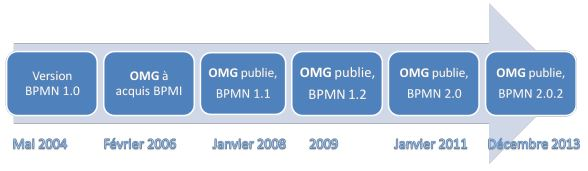
\includegraphics[width=0.82\textwidth]{Chap1/images/image3.JPG}
\caption{Historique du BPMN \citep{vonRosing2015bpmn} }
\label{fig:chap2-ifml-symfony}
\end{figure}
\subsubsection{Éléments de base de BPMN}

Un diagramme BPMN est composé d'un ensemble d'éléments graphiques qui permettent de modéliser les activités, les flux, les relations, les données et l'interaction entre ces éléments.

Les différents éléments sont organisés en cinq catégories :

\begin{itemize}
    \item les objets de flux \textit{(Flow Objects)} ;
    \item les objets de connexion \textit{(Connecting Objects)} ;
    \item les partitions \textit{(Swimlanes)} ;
    \item les données ;
    \item les artéfacts \textit{(Artifacts)}.
\end{itemize}

Les différents éléments de BPMN 2.0 sont illustrés dans la figure ci-dessous.

\begin{figure}[H]
    \centering
    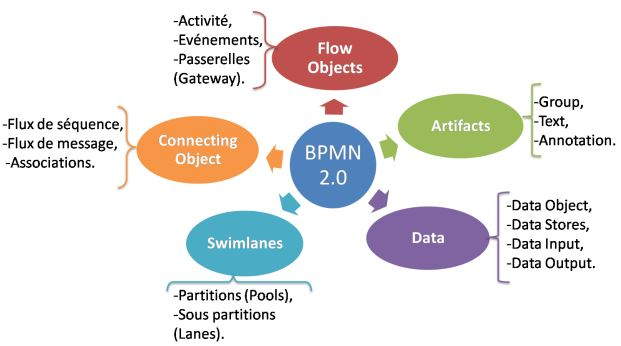
\includegraphics[width=0.75\textwidth]{Chap1/images/image4.JPG}
    \caption{Les différents éléments de BPMN 2.0.}
    \label{fig:elements-bpmn-20}
\end{figure}

\subsubsection*{A. Les objets de flux}

Les objets de flux sont les principaux éléments graphiques qui permettent de définir le comportement d'un processus métier. Il existe trois types d'objets de flux : les activités, les événements et les passerelles.

\textbf{1. Les activités.}
Les activités sont représentées par un rectangle aux coins arrondis. Elles correspondent à une action pouvant être réalisée par un humain ou par une machine. Une activité peut être atomique ou composée. Les principaux types d'activités sont les suivants :

\begin{itemize}
    \item \textbf{Tâche} : une tâche est représentée par un rectangle à coins arrondis tracé avec une seule ligne mince. Elle correspond à une activité atomique ayant un début et une fin. Une tâche ne peut débuter que si la tâche précédente est terminée. Il existe plusieurs types de tâches :
    \begin{itemize}
        \item \textbf{Tâche utilisateur} : elle précise que la tâche est effectuée par un exécutant humain avec l'aide d'une application informatique.
        \item \textbf{Tâche manuelle} : elle précise que la tâche doit être effectuée sans l'aide d'un moteur d'exécution de processus métier ni d'une application. Elle est donc réalisée exclusivement par un acteur humain.
        \item \textbf{Tâche service} : elle utilise un service, qui peut être un service Web ou une application automatisée. Il s'agit d'une tâche automatisée sans intervention humaine.
       % \item \textbf{Tâche d'envoi de message} : elle spécifie l'envoi d'un message à un participant externe au processus. Une fois le message envoyé, la tâche est terminée.
       % \item \textbf{Tâche de réception d'un message} : elle spécifie l'arrivée d'un message provenant d'un participant au processus. Une fois le message reçu, la tâche est terminée.
       % \item \textbf{Tâche script} : elle est exécutée par un moteur de processus métier. Le modélisateur ou l'implémenteur définit un script dans un langage que le moteur peut interpréter. Lorsque la tâche est prête à démarrer, le moteur exécute le script ; lorsque le script est terminé, la tâche est également complétée.
    \end{itemize}

    \begin{figure}[H]
        \centering
        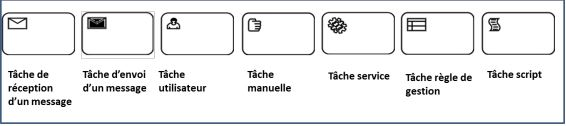
\includegraphics[width=0.9\textwidth]{Chap1/images/image5.JPG}
        \caption{Les types des tâches dans BPMN 2.0.}
        \label{fig:types-taches-bpmn}
    \end{figure}
\end{itemize}

\textbf{2. Les événements.}
Les événements sont représentés par des cercles. Ils correspondent à une action qui survient durant le processus. Ils ont généralement une cause et une conséquence. Il existe trois catégories d'événements : les événements de début, les événements intermédiaires et les événements de fin.

\begin{figure}[H]
    \centering
    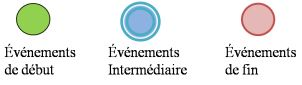
\includegraphics[width=0.65\textwidth]{Chap1/images/image6.JPG}
    \caption{Événements dans BPMN 2.0.}
    \label{fig:evenements-bpmn}
\end{figure}

\begin{itemize}
    \item \textbf{Les événements de début} : ils sont représentés par un cercle avec une seule ligne mince. Ils déclenchent une nouvelle instance de processus. Un processus peut avoir plus d'un événement de début, mais un sous-processus d'événement n'a qu'un seul événement de début.
    \item \textbf{Les événements intermédiaires} : ils sont représentés par un cercle avec une double ligne mince. Ils indiquent une action qui se produit ou peut se produire au cours du processus, entre le début et la fin. Ils peuvent être utilisés pour attraper un déclencheur d'événement et peuvent être placés dans le flux ou à la limite d'une activité.
    \item \textbf{Les événements de fin} : ils sont représentés par un cercle avec une ligne épaisse. Ils marquent la fin de l'instance de processus et ne possèdent pas de flux de séquence sortant.
\end{itemize}

%\begin{itemize}
    %\item \textbf{L'événement de message} : un message est un moyen spécifique de transmission de données d'un processus à l'autre. Le type message signifie l'envoi ou la réception d'un message.
    %\item \textbf{L'événement de minuterie} : il est utilisé pour signifier l'attente d'une condition de temps spécifique pour se déclencher, lancer un processus, un événement ou un sous-processus.
    %\item \textbf{L'événement de condition} : ce type d'événement est déclenché lorsqu'une condition devient vraie. Une condition est un type d'expression.
    %\item \textbf{L'événement d'annulation} : il signale la fin du processus et annule les transactions en cours.
    %\item \textbf{L'événement de compensation} : il signale qu'une tâche doit être annulée. Ce type d'événement permet de définir la tâche utilisée pour compenser une tâche particulière.
    %\item \textbf{L'événement de signal} : il est utilisé pour indiquer l'envoi ou la réception d'un signal.
    %\item \textbf{L'événement de terminaison} : il correspond à l'événement « stop everything ». Lorsqu'un événement de terminaison est atteint, la totalité du processus est arrêtée.
%\end{itemize}

\textbf{3. Les passerelles.}
Les passerelles, ou branchements \textit{(Gateways)}, sont représentées par un losange. Elles servent à représenter les conditions de routage entre les flux d'entrée et les flux de sortie. Les signes internes indiquent le type de contrôle du comportement du branchement.

\begin{figure}[H]
    \centering
    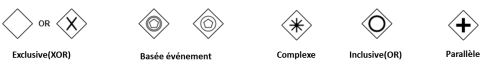
\includegraphics[width=0.9\textwidth]{Chap1/images/image7.JPG}
    \caption{Les branchements de BPMN 2.0.}
    \label{fig:passerelles-bpmn}
\end{figure}

Les différents branchements possibles sont :

\begin{itemize}
    \item \textbf{Exclusive (XOR)} : elle est utilisée pour créer des chemins alternatifs dans un flux de processus. Lors de la scission, elle dirige le flux vers une branche sortante. Lors de la fusion, elle attend qu'une branche entrante se termine avant de déclencher le flux de sortie.
    \item \textbf{Inclusive (OR)} : elle peut être utilisée pour créer des chemins alternatifs parallèles. Contrairement à la passerelle exclusive, toutes les expressions de condition sont évaluées. Lors de la scission, elle active une ou plusieurs branches. Lors de la fusion, elle attend que toutes les branches entrantes se terminent avant de fusionner.
    %\item \textbf{Complexe} : un ou plusieurs chemins sont choisis selon la condition de la passerelle.
    \item \textbf{Parallèle (AND)} : elle est utilisée pour synchroniser et créer des flux parallèles. Lors de la scission, elle active toutes les branches sortantes simultanément. Lors de la fusion, elle attend que toutes les branches entrantes se terminent.
\end{itemize}

\subsubsection*{B. Les objets de connexion}

Les objets de connexion sont les éléments graphiques qui permettent de relier les objets de flux les uns aux autres pour représenter le cheminement du processus. Il existe trois types d'objets de connexion.

\begin{itemize}
    \item \textbf{Les flux de séquence} : ils sont représentés par une flèche pleine et une ligne solide. Ils indiquent l'ordre d'exécution des actions, des événements ou des activités.
\end{itemize}

\begin{figure}[H]
    \centering
    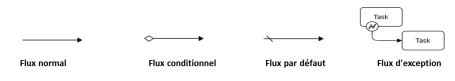
\includegraphics[width=0.85\textwidth]{Chap1/images/image8.JPG}
    \caption{Les flux de séquence de BPMN 2.0.}
    \label{fig:flux-sequence-bpmn}
\end{figure}

\begin{itemize}
    \item \textbf{Les flux normaux} : le flux normal fait référence aux chemins du flux de séquence qui ne commencent pas à partir d'un événement intermédiaire attaché à la limite d'une activité.
   % \item \textbf{Les flux conditionnels} : ils correspondent à des flux de séquence dont l'exécution dépend d'une condition.
    %\item \textbf{Les flux par défaut} : ils sont employés pour les passerelles exclusives ou inclusives. Ce type de flux est utilisé uniquement si tous les autres flux conditionnels sortants ne sont pas vrais au moment de l'exécution du processus.
    \end{itemize}

%\begin{itemize}
    %\item \textbf{Les flux de message} : ils sont représentés par une ligne pointillée avec un cercle ouvert au début et une flèche vide à la fin. Ils correspondent à un lien entre deux processus séparés.
    %\item \textbf{Les associations} : une association est dessinée avec une ligne pointillée. Elle permet de lier des données ou des documents aux objets du processus.
%\end{itemize}

\subsubsection*{C. Les partitions}

Les partitions sont les éléments graphiques permettant de structurer et de regrouper les différents éléments qui composent le diagramme BPMN. Les deux types d'objets sont les participants et les couloirs.

\begin{itemize}
    \item \textbf{Les participants (Pool)} : un pool est la représentation graphique d'un participant à une collaboration. Un participant peut être une entité partenaire spécifique, par exemple une entreprise, ou un rôle partenaire plus général, comme un acheteur, un vendeur ou un fabricant. Un pool peut avoir des détails internes sous forme d'un processus exécuté ou ne présenter aucun détail interne ; dans ce cas, il est considéré comme une « boîte noire ».
    \item \textbf{Les couloirs (Lane)} : un couloir est un rectangle aux coins carrés pouvant être vertical ou horizontal. Il constitue une partition en sous-ensemble dans le pool. Les couloirs sont utilisés pour organiser et classer les activités. Pour illustrer les échanges entre deux couloirs, on utilise des flux de messages.
\end{itemize}

%Un pool est un rectangle à coins carrés tracé avec une seule ligne continue. L'étiquette du pool peut être placée à n'importe quel endroit et dans n'importe quelle direction à l'intérieur, mais doit être séparée du contenu par une seule ligne.

\begin{figure}[H]
    \centering
    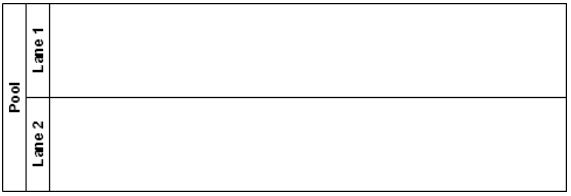
\includegraphics[width=0.55\textwidth]{Chap1/images/image9.JPG}
    \caption{La représentation d'un pool avec deux lanes en BPMN 2.0.}
    \label{fig:pool-bpmn}
\end{figure}

\subsubsection*{D. Les données}

Les données sont utilisées pour expliquer quelles informations sont nécessaires dans le diagramme.

\begin{figure}[H]
    \centering
    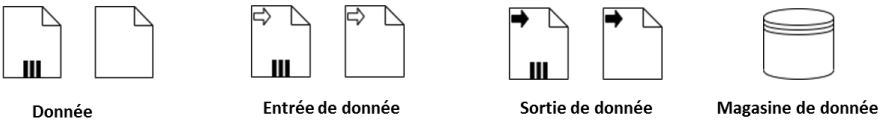
\includegraphics[width=0.75\textwidth]{Chap1/images/image11.JPG}
    \caption{Les données de BPMN 2.0.}
    \label{fig:donnees-bpmn}
\end{figure}

\begin{itemize}
    \item \textbf{Données (Data)} : objets utilisés pour représenter les données nécessaires à l'exécution d'une activité, ainsi que celles produites. Les objets de données peuvent représenter un objet singulier ou une collection d'objets.
   % \item \textbf{Une collection d'objets de données} : elle représente une collection d'éléments de données liés à la même entité de données, par exemple une liste d'articles à commander.
    \item \textbf{Entrée de données (Data Input)} : elle correspond à une entrée externe pour l'ensemble du processus, pouvant être lue par une activité.
    \item \textbf{Sortie de données (Data Output)} : elle correspond au résultat de l'ensemble du processus.
   % \item \textbf{Magasin de données (Data Store)} : il fournit un mécanisme de stockage de données où le processus peut lire ou écrire des données, comme une base de données ou un classeur d'archivage. Il persiste au-delà de la durée de vie de l'instance de processus.
\end{itemize}

\subsubsection*{E. Les artéfacts}

Les artéfacts sont des objets supplémentaires qui apportent des détails complémentaires afin d'assurer une meilleure compréhension du processus. Il existe deux types d'artéfacts : le groupe et l'annotation textuelle.

\begin{figure}[H]
    \centering
    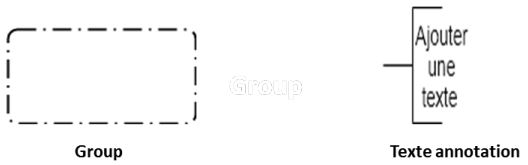
\includegraphics[width=0.5\textwidth]{Chap1/images/image12.JPG}
    \caption{Les artéfacts.}
    \label{fig:artefacts-bpmn}
\end{figure}

\begin{itemize}
    \item \textbf{Groupe} : un groupe est un rectangle à coins arrondis tracé avec une ligne pointillée continue. Il permet de regrouper des tâches d'une même catégorie afin de mieux les repérer visuellement sur le diagramme.
    \item \textbf{Annotation textuelle} : elle permet d'ajouter des commentaires pour faciliter la lecture du diagramme BPMN.
\end{itemize}

\subsubsection{Types de diagrammes BPMN}

BPMN distingue principalement les diagrammes de processus, les diagrammes de collaboration et les diagrammes de chorégraphie \cite{omg2013bpmn}. 
\begin{itemize}
    \item Le \textbf{diagramme de processus} décrit le déroulement interne d'un processus dans un participant donné. Il est adapté lorsque l'on souhaite comprendre l'enchaînement des activités d'un service ou d'un système.
        \begin{figure}[H]
            \centering
            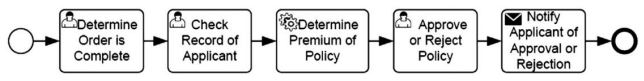
\includegraphics[width=0.65\textwidth]{Chap1/images/image15.JPG}
            \caption{Exemple de diagramme de processus}
            \label{fig:artefacts-bpmn}
            \end{figure}
    \item Le \textbf{diagramme de collaboration} met en relation plusieurs participants et montre les messages qu'ils échangent. Les Pools sont définis comme étant les participants de cette collaboration. Les messages échangés entre les participants sont présentés à l’aide des flux de messages qui connecte deux pools (ou les objets au sein des pools).
        \begin{figure}[H]
            \centering
            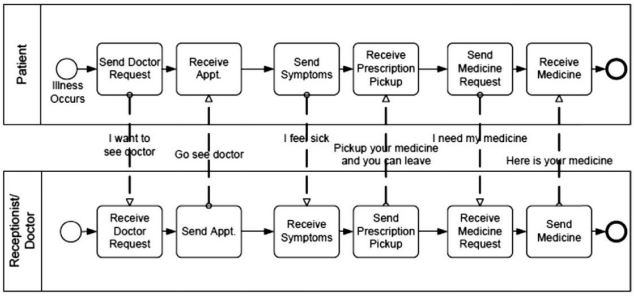
\includegraphics[width=0.65\textwidth]{Chap1/images/image14.JPG}
            \caption{Exemple de diagramme de collaboration}
            \label{fig:artefacts-bpmn}
        \end{figure}
    \item Le \textbf{diagramme de chorégraphie}  se concentre davantage sur les interactions entre participants que sur l'organisation interne de chacun.  Dans ce type de modélisation, la focalisation n’est pas sur l’orchestration (c’est-à-dire sur la manière dont le travail est accompli selon le point de vue des participants), mais sur les échanges de Messages entre les Participants.
        \begin{figure}[H]
            \centering
            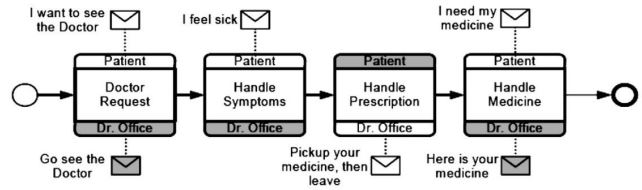
\includegraphics[width=0.65\textwidth]{Chap1/images/image13.JPG}
            \caption{Exemple de diagramme de chorégraphie}
            \label{fig:artefacts-bpmn}
        \end{figure}
\end{itemize}

\mySection{Ingénierie dirigée par les modèles}{}
\label{sec:service_composition}

\subsection{Principe général de l’ingénierie dirigée par les modèles}

L'ingénierie dirigée par les modèles (IDM) désigne une démarche de développement dans laquelle le modèle devient un artefact de travail central. Le modèle n'est donc pas seulement un dessin destiné à expliquer une idée : il sert à décrire un système à un niveau d'abstraction choisi, à vérifier certains choix, à organiser les connaissances du domaine et, lorsque l'outillage le permet, à produire d'autres modèles ou des artefacts techniques. Cette approche répond principalement à deux difficultés du génie logiciel : la croissance de la complexité des systèmes et l'évolution rapide des technologies. En plaçant les modèles au centre du développement, l'IDM cherche à mieux séparer les préoccupations, à réduire la dépendance immédiate aux détails techniques et à rendre certaines tâches répétitives plus maîtrisables \cite{jezequel2012,meghzili2022}.  L'objectif n'est pas de supprimer l'intervention humaine, mais de déplacer une partie de l'effort vers des modèles explicites, contrôlables et transformables.

\subsection{Notion de base en Ingénierie Dirigée par les Modèles}

Un système est l'entité étudiée. Il peut être composé d'éléments reliés entre eux, posséder une organisation interne et interagir avec son environnement. Dans l'IDM, le système n'est généralement pas manipulé directement dans toute sa complexité ; il est représenté par un ou plusieurs modèles.

Un modèle est une abstraction d'un système, construite dans un objectif donné. Il retient les informations utiles pour répondre à certaines questions, tout en laissant de côté les détails qui ne sont pas nécessaires au point de vue choisi. Cette idée est importante : un modèle n'a pas vocation à tout contenir. Sa valeur dépend de sa pertinence par rapport au besoin d'analyse, de conception ou de vérification. Jézéquel, Combemale et Vojtisek définissent ainsi le modèle comme un ensemble de faits caractérisant un aspect d'un système selon un objectif précis \cite{jezequel2012}.

Un méta-modèle définit le langage dans lequel les modèles sont exprimés. Il précise les concepts autorisés, leurs relations et les contraintes qui structurent les modèles valides. Le méta-modèle joue donc un rôle de cadre : il rend les modèles manipulables par des outils, car il décrit leur structure attendue. Au-dessus, le méta-méta-modèle fournit le langage permettant de définir les méta-modèles. L'Object Management Group (OMG) organise cette logique selon quatre niveaux : M0 pour le système réel, M1 pour les modèles, M2 pour les méta-modèles et M3 pour le méta-méta-modèle, généralement associé à MOF, Meta-Object Facility \cite{jezequel2012,omgmof}.

\begin{figure}[H]
    \centering
    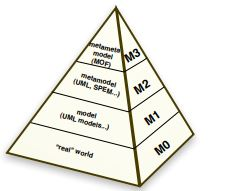
\includegraphics[width=0.50\textwidth]{Chap1/images/image19.JPG}
    \caption{Pyramide de modélisation de l'OMG.\cite{jezequel2012}.}
    \label{fig:artefacts-bpmn}
\end{figure}

\subsection{Transformation de modèles}

La transformation de modèle consiste à produire un modèle cible à partir d'un modèle source, selon des règles définies. Ces règles décrivent les correspondances entre les éléments du modèle d'origine et ceux du modèle obtenu. Une transformation peut être endogène lorsque les modèles source et cible sont conformes au même méta-modèle ; elle est exogène lorsqu'ils relèvent de méta-modèles différents. Elle peut aussi être horizontale lorsqu'elle reste au même niveau d'abstraction, ou verticale lorsqu'elle fait évoluer le niveau d'abstraction, par raffinement ou par abstraction \cite{jezequel2012,idm2020}.

Les transformations occupent une place centrale dans l'IDM parce qu'elles donnent un caractère productif aux modèles. Elles peuvent servir à raffiner une spécification, restructurer une représentation, migrer d'une technologie à une autre, générer du texte ou produire du code. Les deux grandes familles généralement retenues sont les transformations modèle-vers-modèle (M2M) et modèle-vers-texte (M2T). Les standards et langages de transformation, comme QVT, ATL ou les approches par templates, cherchent à formaliser ces passages afin qu'ils soient reproductibles et moins dépendants d'une manipulation manuelle \cite{jezequel2012,omgqvt}.

\begin{figure}[H]
    \centering
    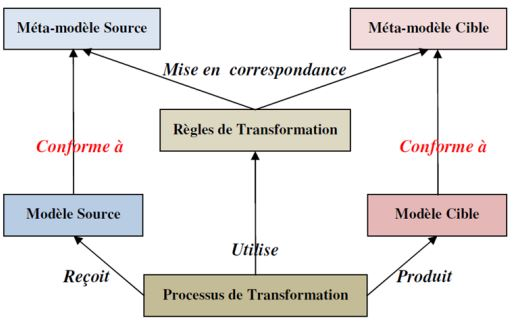
\includegraphics[width=0.65\textwidth]{Chap1/images/image16.JPG}
    \caption{Schéma de base d'une transformation de modèle  \cite{meghzili2022}}
    \label{fig:artefacts-bpmn}
\end{figure}

\subsection{Model-Driven Architecture}

La Model-Driven Architecture (MDA) est une initiative de l'OMG qui applique les principes de l'IDM à l'architecture logicielle. Elle vise à décrire une application en distinguant les modèles indépendants de la plateforme et les modèles liés à une plateforme particulière.
\begin{figure}[H]
    \centering
    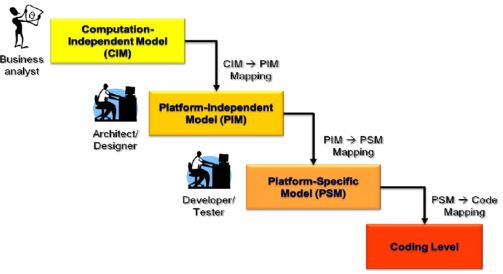
\includegraphics[width=0.65\textwidth]{Chap1/images/image17.JPG}
    \caption{Illustration des trois niveaux d'abstraction du MDA  \cite{meghzili2022}}
    \label{fig:artefacts-bpmn}
\end{figure}
\begin{itemize}
    \item \textbf{CIM \textit{(Computation Independent Model)}} : il décrit les besoins métier et
    les objectifs sans se préoccuper des aspects techniques. C'est le niveau où l'on
    formalise ce que le système doit faire, indépendamment de la façon dont il sera
    implémenté.

    \item \textbf{PIM \textit{(Platform Independent Model)}} : ce modèle représente l'architecture
    et les fonctionnalités du système sans faire référence à une technologie ou une
    plateforme donnée. Il constitue un pont entre les exigences métier et la solution
    technique.

    \item \textbf{PSM \textit{(Platform Specific Model)}} : il traduit le PIM en une implémentation
    concrète, en intégrant les contraintes et les choix technologiques spécifiques
    comme le framework, le langage ou l'environnement d'exécution.
\end{itemize}

L'intérêt de la MDA est de préserver les décisions de conception à un niveau moins fragile que le code. Lorsque les technologies changent, les modèles indépendants peuvent être conservés plus longtemps, tandis que les transformations et les modèles spécifiques sont adaptés aux nouvelles plateformes. La MDA ne se limite donc pas à une génération automatique de code ; elle propose une organisation du développement où la séparation entre abstraction, plateforme et implémentation devient explicite.

\mySection{Applications web métier}{}
\label{sec:service_composition}

\subsection{Généralités sur le développement web}

\subsubsection{Historique du développement web}

Le développement web est né avec un objectif essentiellement documentaire :
publier des informations et permettre leur consultation à distance. Dans cette
première logique, le navigateur demandait une page, le serveur retournait un
document HTML, puis le navigateur l'affichait. Les fondements du Web restent
liés à cette organisation : identification des ressources, liens hypertextes,
représentations et échanges entre clients et serveurs \cite{w3c2004webarch}.

L'évolution des usages a progressivement transformé le Web en plateforme
applicative. Les pages statiques ont été complétées par des formulaires, des
espaces authentifiés, des tableaux de bord, des services de paiement, des
plateformes universitaires et des applications administratives. Le navigateur
n'est alors plus seulement un lecteur de documents ; il devient l'interface
d'un système logiciel distant. Cette évolution a donné plus d'importance aux
langages côté client, aux serveurs d'application, aux bases de données, aux API,
à la sécurité et à la maintenabilité.

HTTP demeure le support principal de ces échanges. Le RFC 9110 le définit comme
un protocole applicatif fondé sur des requêtes, des réponses et des méthodes
comme \texttt{GET}, \texttt{POST}, \texttt{PUT}, \texttt{PATCH} ou
\texttt{DELETE} \cite{rfc9110}. Cette base explique pourquoi les applications
web modernes sont généralement construites autour de routes, de ressources,
d'opérations métier et de formats de représentation comme HTML ou JSON.

\subsubsection{Définition d'application web et concepts du web}

\subsubsection*{Définition}

Une application web peut être définie comme un logiciel accessible à partir d’un
navigateur ou d’un client reposant sur les technologies du Web. Contrairement à
un site essentiellement informatif, elle prend en charge des interactions avec
l’utilisateur, traite des données, applique des règles métier et produit des
résultats exploitables. Ainsi, une plateforme de demande d’attestation ne se
limite pas à afficher des pages : elle permet de soumettre une demande, de suivre
son état, de contrôler les droits d’accès et de générer un document. Elle relève
donc pleinement d’une application web métier.

\subsubsection*{Concepts du web}

La conception d’une application web repose sur des choix architecturaux qui
influencent directement sa maintenabilité, son évolutivité et la séparation des
responsabilités. Le modèle client-serveur constitue la base de ce fonctionnement :
le client, généralement un navigateur, transmet les actions de l’utilisateur,
tandis que le serveur traite les requêtes, accède aux données et retourne les
réponses appropriées \cite{mdn2026webworks}. Cette séparation est particulièrement
importante dans les applications métier, où plusieurs utilisateurs interagissent
avec les mêmes ressources selon des droits et des règles différents.

Pour améliorer l’organisation interne du système, les applications web modernes
s’appuient souvent sur une architecture en couches. La couche de présentation
gère les interfaces et les formulaires, la couche métier applique les règles du
domaine, et la couche d’accès aux données assure la communication avec la base.
Cette structuration limite le couplage entre les composants et facilite les
évolutions du système. Le patron Modèle-Vue-Contrôleur s’inscrit dans cette
logique en distinguant les données et règles du domaine, leur présentation à
l’utilisateur et le traitement des actions déclenchées par celui-ci
\cite{leff2001web}.

Dans les architectures récentes, les applications monopages
\textit{(Single Page Applications)} renforcent la séparation entre le client et
le serveur en confiant une partie importante de l’interface au navigateur. Elles
offrent une expérience plus fluide, mais exigent une maîtrise accrue de la
complexité du frontend, notamment lorsque l’application doit représenter des
tâches, des états de dossier ou des actions liées à un processus métier
\cite{mdn2026spa}. Les API web jouent alors un rôle central en exposant les
fonctionnalités du système sous forme de ressources accessibles, comme
\texttt{/demandes}, \texttt{/documents} ou \texttt{/taches}. Le style REST,
formalisé par Fielding, a fortement contribué à cette organisation des échanges
autour des ressources, des représentations et d’interactions sans état
\cite{fielding2000architectural}.

Ainsi, le développement d’une application web ne consiste pas seulement à produire
des interfaces. Il implique de définir une architecture capable d’articuler
présentation, logique métier, persistance des données et échanges entre
composants. Cette base conceptuelle est essentielle pour comprendre les
applications web orientées processus, dont le comportement dépend étroitement de
l’évolution du workflow.

\subsubsection{Frameworks d'application web}

Un framework d'application web fournit un cadre de développement, des composants
réutilisables et des conventions pour construire une application. Il évite de
réécrire à chaque projet les mêmes mécanismes : routage, contrôleurs, accès aux
données, gestion des sessions, validation, rendu des vues, authentification ou
traitement des erreurs. Son intérêt n'est pas seulement de gagner du temps ; il
permet aussi d'organiser le code de manière plus régulière et plus maintenable.

\subsubsection*{Frameworks de développement web back-end}

Les frameworks back-end structurent la partie serveur de l'application. Ils
organisent les routes, les contrôleurs, les services, les modèles de données et
les mécanismes de sécurité. Dans une application métier, c'est dans cette partie
que sont vérifiées les règles comme l'autorisation d'un utilisateur, la validité
d'une demande ou le passage d'un dossier d'un état à un autre. Ils peuvent aussi
faciliter l'accès aux bases de données, la journalisation, la gestion des erreurs
et l'exposition d'API. Des environnements comme Spring, Django, Laravel ou
Express illustrent cette famille d'outils.

\subsubsection*{Frameworks de développement web front-end}

Les frameworks front-end structurent l'interface exécutée dans le navigateur. Ils
aident à construire des composants réutilisables, gérer les formulaires,
afficher les données et réagir aux actions de l'utilisateur. Dans une application
orientée processus, cette partie est importante parce qu'elle rend visibles les
tâches à traiter, les états du dossier, les messages d'erreur et les actions
autorisées. Leur rôle est donc aussi ergonomique : ils aident à présenter le
workflow de façon compréhensible pour chaque acteur. Des outils comme Angular,
React ou Vue.js sont représentatifs de cette logique côté client.

\subsubsection{Sécurité dans les applications web}

Les politiques de contrôle d’accès permettent de définir les règles qui encadrent
l’accès aux informations au sein d’une entreprise. Dans les applications web, elles
contribuent à sécuriser la manipulation des données sensibles, notamment les
données des utilisateurs. Parmi ces politiques, le modèle RBAC, ou contrôle
d’accès basé sur les rôles, est largement utilisé, car il permet d’organiser les
droits d’accès en fonction des responsabilités attribuées aux utilisateurs.

Le principe du RBAC consiste à associer des permissions à des rôles, puis à
affecter les utilisateurs aux rôles correspondant à leurs besoins. Cette approche
simplifie la gestion de la sécurité, car les administrateurs peuvent créer des rôles,
leur attribuer des autorisations et contrôler ainsi l’accès aux ressources. Elle
favorise également des principes essentiels comme le moindre privilège, la
séparation des tâches et la protection des informations sensibles.

\begin{figure}[H]
    \centering
    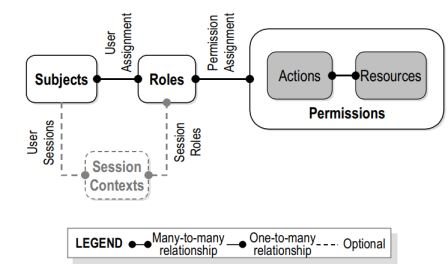
\includegraphics[width=0.65\textwidth]{Chap1/images/image20.JPG}
    \caption{Coeur du modèle RBAC  \cite{yuan2005abac}}
    \label{fig:artefacts-bpmn}
\end{figure}

\subsection{Applications web métier}

\subsubsection{Définitions et principe}

Une application web orientée processus, ou \textit{process-aware web
application}, est une application dont le comportement est organisé autour d'un
processus métier explicite. Les écrans, les actions disponibles, les rôles des
utilisateurs et les changements d'état suivent l'avancement d'un workflow. Cette
idée rejoint la définition des systèmes d'information orientés processus, dans
lesquels les activités, les acteurs et les règles d'enchaînement occupent une
place centrale \cite{dumas2018fundamentals,weske2012bpm}.

Dans une application classique, le développeur peut coder directement les
conditions de passage d'un état à un autre. Dans une application orientée
processus, ces passages sont plutôt décrits par un modèle, souvent en BPMN. Le
modèle précise les tâches à réaliser, les décisions possibles, les événements
attendus et les responsabilités des acteurs. L'application web fournit ensuite
les interfaces, les services et les données nécessaires à l'exécution concrète
de ce processus.


\subsubsection{Moteur de processus}

Un moteur de processus est un composant logiciel chargé d'exécuter un modèle de
processus. Lorsqu'un processus BPMN exécutable est déployé, il peut créer des
instances, enregistrer leurs variables, distribuer des tâches humaines,
déclencher des services automatiques et suivre l'historique d'exécution
\cite{camunda2026modeler}. Il joue donc un rôle d'orchestration : il indique ce
qui doit être fait, par qui, à quel moment et selon quelles conditions.

Dans une application web orientée processus, le moteur ne remplace pas le
frontend, le backend ni la base de données. Il coordonne le déroulement du
travail. Le frontend permet aux utilisateurs d'interagir avec les tâches, le
backend applique les règles propres à l'application et dialogue avec le moteur,
tandis que la base de données conserve les informations métier. Cette
répartition évite de confondre l'exécution du workflow avec la construction
complète de l'application.

\mySection{Conclusion}{}

Dans ce chapitre, nous avons présenté les concepts nécessaires à la suite du
mémoire : processus métier, BPM, BPMN, développement web et applications web
métier. Nous avons montré qu'un modèle BPMN peut guider
l'organisation du travail, mais qu'une application web doit aussi gérer
l'interface, les données, la sécurité et l'exécution technique. Le chapitre
suivant s'appuie sur ces bases pour analyser les travaux existants.
